

\section{Fixing the Inefficiencies}
\label{sec:opt}

After identifying the performance inefficiencies in the \numpactions problematic actions across the 12 studied applications, we manually fix each of them and measure how much our fixes improve the performance of the corresponding application webpages. Our goal is to quantify the importance of the anti-patterns discussed in Section \ref{sec:causes}. 

\subsection{Methodology}
We use the same 20,000-record database configuration used in profiling to measure performance improvement.
For a problematic action that contains multiple inefficiency problems, we fix one at a time and report the speedup for each individual fix.
To fix API-use problems, we change model/view/control files that are related to the problematic API uses; to add missing indexes or fields, we change corresponding Rails migration files; to apply pagination, we use the standard \texttt{will\_paginate} library~\cite{gem:paginate}. We carefully apply  fixes to make sure we do not change the program semantics.
Finally, for two actions in Lobster, we eliminate the expensive checking about whether to show user guidelines, as discussed in Section \ref{sec:simplifyfeatures}.
%We will accumulate the optimization step by step. For example, $HomeController.recent$ action is slowed down by two redundant computation called \texttt{r1} and \texttt{r2}, after optimization \texttt{o1} which removes removing \texttt{r1}, the execution time is reduced from 3782 to 2045, and after optimization \texttt{o2} which removes \texttt{r2}, the execution is reduced from 2045 to 1013. As a result, the speed-up of \texttt{o1} is 1.8 $\times$, and the speed-up of \texttt{o2} is 2 $\times$. We will count \texttt{o1} and \texttt{o2} separately in Figure \ref{speedup}.
\begin{figure}
\centering
\label{fig:sl}
\begin{subfigure}
% \subfigure[Server-time speedup ($\times$)]{
\centering
    \includegraphics[width=0.4\linewidth]{hownotto/speedup}
   \caption{Server-time speedup ($\times$)}
    \label{fig:speedup}
\end{subfigure}
% }
% \subfigure[Line of code changes]{
\begin{subfigure}
    \centering
    \includegraphics[width=0.4\linewidth]{hownotto/loc}
   \caption{Line of code changes}
    \label{fig:loc}       
\end{subfigure}
% }
\caption{Performance fixes and LOC involved}
\end{figure}

\subsection{Results}
In total, \numacissues fixes are applied across 39 problematic actions \footnote{Among the 40 problematic actions identified by our profiling, 1 of them (from GitLab) spends most of its time in file-system operations and  cannot be sped up unless its core functionality is modified. 
} to solve the \numacissues problems listed in Table \ref{tab:freq}.
\vspace{-0.08in} 
\paragraph{\bf Speedup of the fixes}
Figure \ref{fig:speedup} shows the amount of server-time speedup and the sources of the speedup broken down into different anti-patterns as discussed in Section \ref{sec:causes}.

Many fixes are very effective. About a quarter of them achieve more than 5$\times$ speedup, and more than 60\% of them achieve more than 2$\times$ speedup. Every type of fixes
has at least one case where it achieves more than 2$\times$ speedup. 
%Although never providing more than 5X speedups, changing loading strategy provides more than 4X speedups in four cases. 
The largest speed-up is around 39 $\times $ achieved by removing unnecessary feature in \texttt{StoriesController.new} action in Lobsters, i.e., the example we discussed in Section \ref{sec:simplifyfeatures}. 

There are 40 fixes that alter neither the display nor the functionality of the original application. That is, they fix the anti-patterns discussed in Section \ref{causes:api} and \ref{causes:db}. They
achieve
an average speedup of 2.2$\times$, with a maximum of 9.2$\times$ speedup by adding missing fields in \texttt{GanttsController.show} from Redmine.

For all 39 problematic actions, many of which benefit from more than one fix, their average server time is reduced from \serverbefore seconds to \serverafter seconds, and the corresponding end-to-end page loading time is reduced from \eoebefore seconds to \eoeafter seconds, including client rendering and network communication. In other words, by writing code that contains the anti-patterns discussed earlier, developers degrade the performance of their applications by about $6\times$.
%\shan{we probably also should report the total server time and end-to-end time of the 44 actions before and after the optimization. do you have that figure?}

We have reported these 64 fixes to corresponding developers. So far, we have received developers' feedback for \numconfirmedpaissues of them, all of which have been confirmed to be true performance problems and \numfixedpaissues have already been fixed based on our report.%\shan{TODO: discuss why many have no feedback?}\junwen{For those related to API design, maybe it's hard for developers to give answer soon}
\vspace{-0.08in} 
\paragraph{\bf Simplicity of the fixes}
Figure \ref{fig:loc} shows the lines of code changes required to implement the fixes. 
The biggest change takes 56 lines of code to fix (for an inefficient rendering (IR) anti-pattern), while the smallest change requires only 1 line of code in 27 fixes. More than 78\% of fixes require fewer than 5 lines. In addition, among the fixes that improve performance by 3$\times$ or more, more than 90\% of them take fewer than 10 lines of code. Around 60\% of fixes are intra-procedural, involving only one function.  
%\shan{hmm, the lines of code are actually bigger than i expected. need discussion.}\shan{please also report inter-procedural changes vs intra-procedural changes.} 
\begin{comment}
\begin{figure}[h]
  \centering
  \includegraphics[width=1\columnwidth]{figs/speedup}
  \caption{Application server-time speedup after fixes\shan{to fix anti-pattern captions later, same for next figure}\junwen{done}
  }

  \label{speedup}
\end{figure}

\begin{figure}[h]
  \centering
	\includegraphics[width=1\columnwidth]{figs/loc}
  \caption{Lines of code in performance fixes \alvin{move legend into the graph? I think we have room}}

  \label{locchange}
\end{figure}
\end{comment}


These results quantitatively show that there is still a huge amount of inefficiency in 
real-world ORM applications. Much inefficiency can be removed through few lines of code changes.
 A lot of the fixes can potentially be automated, as we will discuss in Section \ref{sec:dis}.

\begin{comment}
\subsection{Automate Solutions}
\subsubsection{How complex are the changes that developers apply to optimize their programs}

\textbf{  Loc change}
\textbf{  program complexity change}

\subsubsection{Are there common patterns can be automated}

\end{comment}